
\subsection{Módulo de planimetría}

% A- Módulo de planimetría
% - Objetivo del módulo	
El objetivo de este módulo es caracterizar el escenario donde transcurre el experimento. Actualmente las trayectorias en Navindoor se centran en el desplazamiento en interiores, por lo que se ofrece las herramientas básicas para caracterizar un edificio de varias plantas. Esta caracterización nos proveerá información sobre las restricciones de movimiento, posición de puntos de acceso, altura entre plantas, etc. Esta información puede ser usada por los modelos generación de trayectorias y señales, además de los algoritmos de localización.
% - Modelización 
%     - Diagrama de clases
%     - nodos, paredes, puertas, ascensores, escaleras, APs, plantas

Se ha diseñado una jerarquía de clases presentado en la figura \ref{fig:esquemabuilding}, que representarán los objetos necesarios para la caracterización de un edificio. Se ha creado la clase \emph{node}, para representar un punto en el espacio tridimensional. A partir de este objeto se construyen las demás clases dentro del módulo de planimetría. Los objetos \emph{walls}, que representa  las paredes del edificio, son construidos a partir de dos objetos \emph{node}. Por otra parte, también existen  elementos puntuales, por lo que se ha creado clases que heredan las propiedades de \emph{node}. Estos son los objetos \emph{stairs}, \emph{elevators}, \emph{doors} y \emph{beacons}. Los objetos \emph{stairs} y \emph{elevators} nos indican los puntos de salida de una planta. Los objetos \emph{doors}, se definen dentro de los objetos \emph{wall}s, y permiten el paso en su entorno. Por último, los objetos \emph{beacons} representan puntos de acceso generadores de señales de radio frecuencia. Los objetos antes mencionados se almacenan en una clase llamada \emph{level} en forma de atributos. Por último se ha creado la clase \emph{building} que en sus atributos contiene un lista de objetos \emph{level}. 
\begin{figure}[!ht]
    \centering
    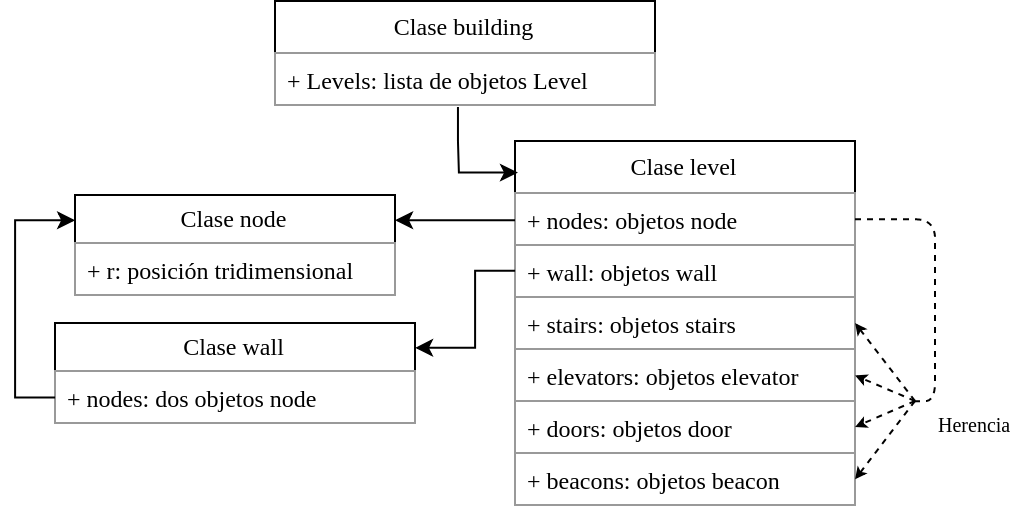
\includegraphics[width=0.8     \columnwidth]{img/Design/planimetria.png} 
    \caption[]{Esquema de la clases.}
    \footnotesize
    Las flechas salientes indican de qué clase es el objeto. Mientras que el listado dentro de cada caja representa las propiedades que contiene una clase. 
    \label{fig:esquemabuilding}
\end{figure}   


% - Explicación básica del proceso de generación de planimetría:  
%     - Clicks con el ratón 
%     - mapa real como plantilla
%     - Visualización 3D
Para la creación de cada uno de estos objetos existe un constructor siguiendo las bases de la programación orientada a objetos, sin embargo la caracterización de la planimetría de esta forma puede ser muy tediosa. Es por ello que se ha optado en el desarrollo de una GUI (figura \ref{fig:interfaz1}), que nos ayude en este trabajo. De esta forma se puede definir objetos \emph{nodes} con simples \emph{clicks}, y paredes uniendo objetos \emph{nodes}. Además la GUI permite cargar imágenes, en formato PNG, de la planimetría de interés dentro del espacio de trabajo. Esto se puede realizar para cada una de las plantas de manera que podamos crear una fiel reproducción de la planimetría utilizando los planos reales como plantillas. Un vez construido la planimetría podemos ver el objeto \emph{building} en 3D, gracias a las opciones de la GUI.


\begin{figure}
    \centering
    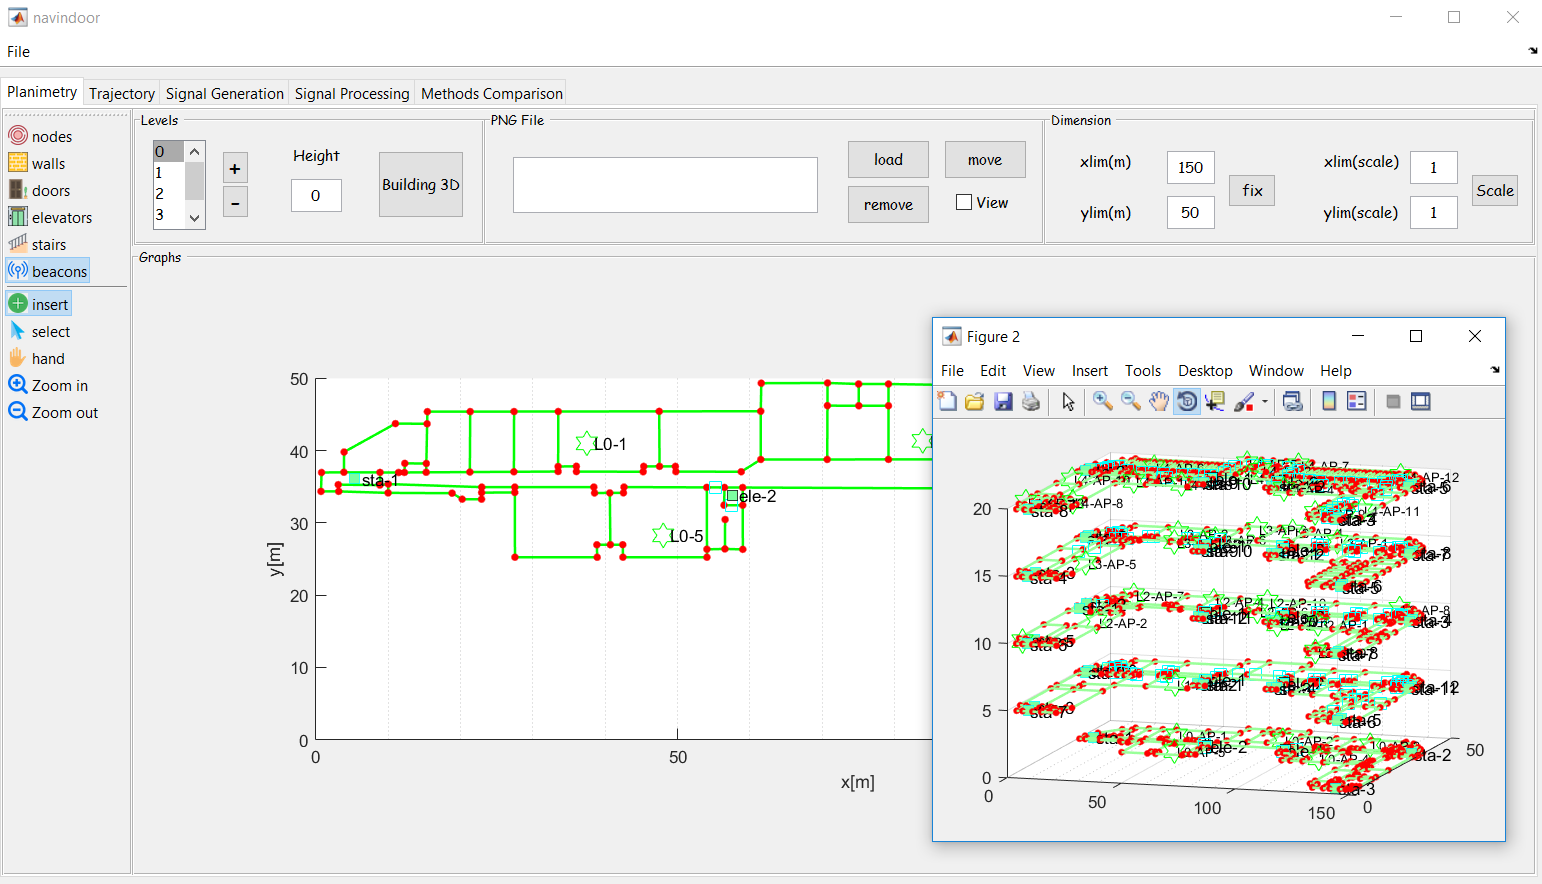
\includegraphics[width=1.00\columnwidth]{img/Design/1.PNG}
    \caption{Interfaz gráfica para el diseño de la planimetría \emph{building}.}
    \footnotesize
    En la imagen se muestra la interfaz con un edificio de cinco plantas. La figura externa es una representación tridimensional del edificio.
    \label{fig:interfaz1}
\end{figure}

% ----------------------------------------------------------------------


